\chapter{模块介绍}
这一章节主要介绍软件的开发过程,将软件按照功能逐步地进行细致划分,从而完成软件的设计任务。
\section{软件框图}
如 \figurename{} \ref{fig:softarch} 为软件整体的关系图。
\begin{figure}[h]
	\centering
	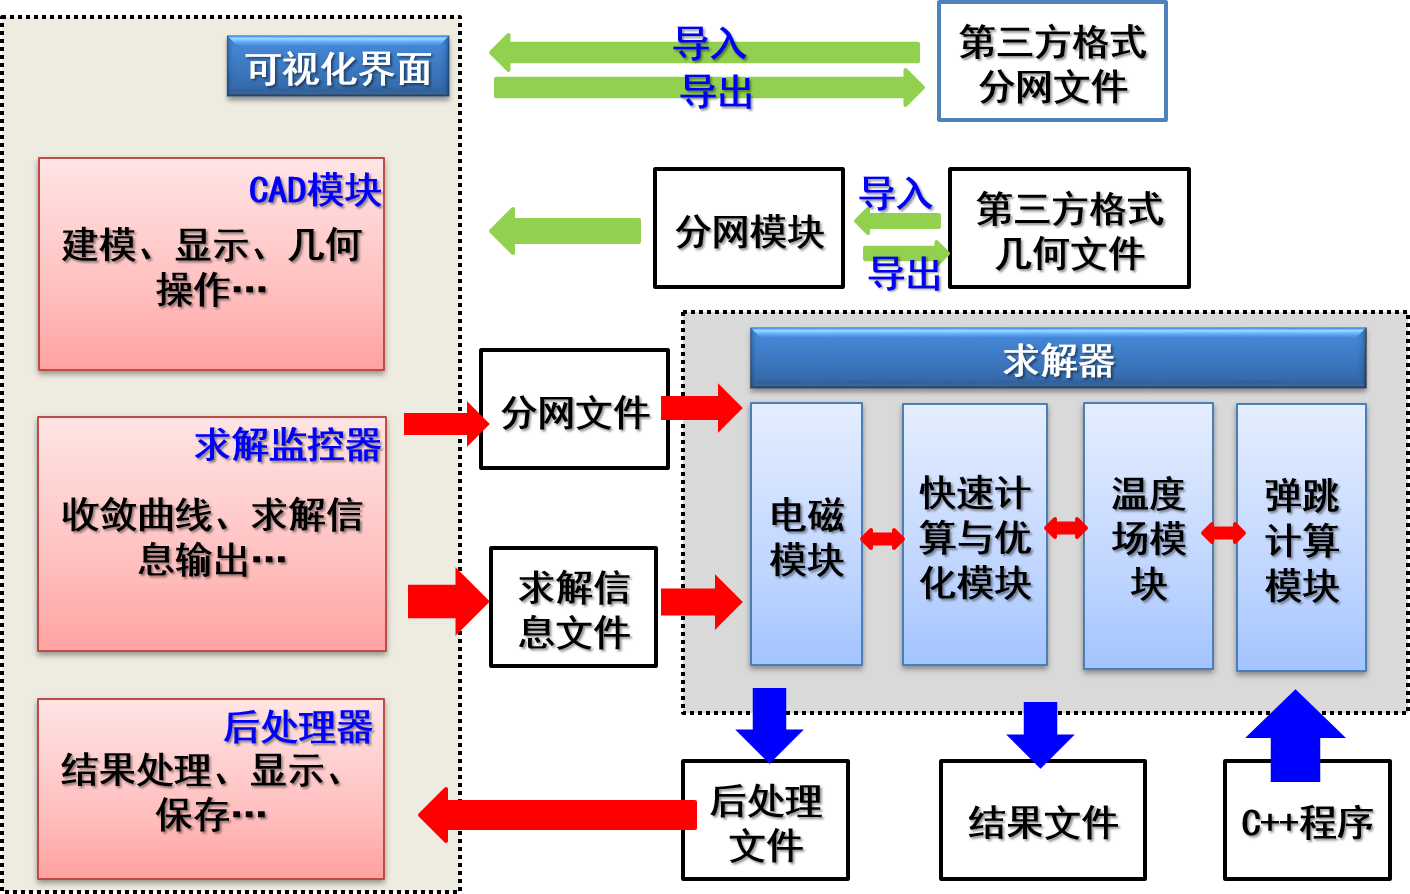
\includegraphics[width=0.7\linewidth]{figures/softarch}
	\caption{软件FEEM整体设计框架}
	\label{fig:softarch}
\end{figure}

\subsection{磁场问题的有限元求解}

\subsection{优化问题}

\section{界面设计}

\subsection{Ribbon模块}

\subsection{QtFLEX模块}

\subsection{界面布局}

\section{定义}
为了对数据进行存储,需要定义合理的格式和存储方式。
\subsection{工程文件格式及存储}
工程文件,即是软件会打开的文件,通过读取这个文件,软件可以获得该项目当中的几何模型、物理设置参数、分网信息、求解信息等。目前,最普遍的方式就是采用标记式语言进行存储,首选XML语言。
\subsection{几何文件格式及存储}
几何图形是用户在操作软件过程当中一直会使用到的东西,所以这部分数据肯定是常驻内存。在软件的核心,需要定义几何存储的格式来代表各种图形,这些图形可以是用户自己创建的,也可以是不同格式的几何文件转换过来的。
\subsection{分网文件格式及存储}
跟几何文件类似,也需要在工程内部自定义分网数据格式,来保存从各种格式的分网文件读取并转换而来的数据。
\subsection{结果数据文件及存储}
在求解结束后,需要一个数据结构来存储计算得到的各种数据结果。
\subsection{编程代码规范}
为了使软件开发尽量的规范,开发小组成员应当遵守以下操作:
\section{CAD绘图}
几何绘图是软件可视化最重要的一个部分。
\subsection{绘图原理}
在显示屏上你所看到的有趣的东西,都是程序员尽力地让一切看起来都跟真的似的,实际上,它依旧还是冷冰冰的机器,只是用的时间长了可能会发热而已。
\subsection{基本几何形状}
需要实现的基本几何形状有:点、线、圆弧、长方形等。
\subsection{形状操作}
所谓的用户能够对显示的几何形状进行控制,实际上是程序针对用户的鼠标操作与实际几何形状的位置进行了比较计算之后,进行了一些算法。每一次改变都会导致显示内容的刷新,只不过肉眼无法辨别出来。
\subsubsection{形状选中、调整大小、删除、隐藏显示}

\subsubsection{自动吸附}

\subsubsection{布尔操作}

\subsubsection{缩放、变形}

\subsection{与分网显示、后处理的接口}

\subsection{参数绘图}

\section{材料库}
为了对模型当中的结构添加相应的材料属性,需要提供一个材料管理器的功能,能够存储一些常见的材料,并且能够实现新建、修改、删除等操作。
\subsection{已有材料库}

\subsection{新建、删除材料}

\subsection{导入、导出材料}

\section{分网生成}
分网无疑是有限元器求解最为关键的步骤之一。
\subsection{分网读取、导出}

\subsection{有限元分网形状}

\subsection{读取几何模型并分网}

\subsection{分网控制}

\subsection{删除分网}

\subsection{分网可视化}

\section{求解器}

\subsection{求解器设置}

\subsection{优化模块}
当所有的求解信息都设置好后,不仅可以实现磁场的求解,还能够实现对某些参数的优化设计。

\subsection{收敛曲线显示}

\section{后处理}
求解器计算得到的结果无疑要使用最好的方式展现给用户。
\subsection{结果曲线}

\subsection{结果云图}

\subsection{结果矢量图}

\subsection{数据导出}